\renewcommand{\inputfile}{\version\ - edited 2007-03-11 symODEs}
% section: Symmetries of dynamical systems
% $Author$ $Date$

\subsection{Definition of symmetry}

We consider a system of \ode's of the form
\beq
	\dot{x} = \vf(x,\lambda)
	\label{eq:difeq}
\eeq
where $\vf: \Rls{n}\times\Rls{r}$ a $C^\infty$ mapping. When
not important we will suppress the $r$-dimensional vector of parameters
$\lambda$ in the notation.

As is well known any compact Lie group acting on $\Rls{n}$ can be identified
with a subgroup of $\On{n}$, \cf\ for example \refref{golubII}
for a sketch of the proof. Therefore, without loss of generality
we will concentrate on subgroups $\Gamma\subseteq\On{n}$ in the following.

\begin{definition}
\label{def:symmetry}
\index{symmetry}
We call a group element $\gamma\in\On{n}$ a symmetry of \refeq{eq:difeq} if for every solution
$x(t)$, $\gamma x(t)$ is also a solution.
\end{definition}

The question now arises on how to check for symmetries of \refeq{eq:difeq} since
we generally do not have knowledge of the set of all solutions. Let $x(t)$ be a solution
of \ref{eq:difeq}. Then by \refDef{def:symmetry} $y(t)=\gamma x(t)$ is another solution 
and therefore satisfies \refneq{eq:difeq}:
\[
 \dot{y}(t)=\vf{y(t)}=\vf(\gamma x(t))\,.
\]
On the other hand
\[
 \dot{y}(t)=\gamma \dot{x} = \gamma \vf(x(t))\,,
\]
for any solution $x(t)$. Since solutions exist for any $x\in\Rls{n}$ we are led to the following 
condition for $\gamma$ to be a symmetry of \refeq{eq:difeq}:
\beq
	\vf(\gamma x) =\gamma \vf(x)
	\label{eq:equiv}
\eeq
for all $x\in\Rls{n}$. We say that $\vf$ \emph{commutes} with $\gamma$ or that $\vf$ is $\gamma$-\emph{equivariant}.
When $\vf$ commutes with all $\gamma\in\Gamma$ we say that $\vf$ is $\Gamma$-equivariant\index{equivariant}.
% When $f$ is $\gamma$-equivariant
% the \ode~ \ref{eq:difeq} remains invariant under the action of $\gamma$.

Clearly the finite time flow $\flow{t}{\gamma x_o}$ through $\gamma x_o$ 
satisfies the equivariance condition $\flow{t}{\gamma x_o}=\gamma \flow{t}{x_o}$ from 
the definition of symmetry and uniqueness of solutions.


\index{Lorenz equations!symmetry}For example, the vector field in Lorenz equations  \refneq{eq:lorenz} is equivariant under the group
$\Zn{2}\cong\Dn{1}$ acting on \Rls{3} by
\[
	\Rot{\pi}(x,y,z) = (-x,-y,z)\,.
\]
Notice that this transformation can be considered as either as rotation by $\pi$ around the $z$ axis (hence the
group \Zn{2}) or as a reflection about the origin in a plane perpendicular to the $z$-axis (hence the group \Dn{1}).

\index{Complex Lorenz equations!symmetry}As another example, the vector field in \CLe~ \refneq{eq:CLe} is equivariant under the group \SOn{2} acting on $\Rls{5}\cong \Clx{2}\times \Rls{}$
by
\beq
 \Rot{\theta} (x,y,z) = (e^{i\theta} x, e^{i\theta} y, z)\,,\ \ \  \theta\in[0,2\pi)\,.
 \label{eq:RotCLe}
\eeq

\index{Armbruster-Guckenheimer-Holmes flow!symmetry}Finally, the symmetry group of the \AGHe~\refneq{eq:AGH} is \On{2} acting by
\begin{eqnarray*}
  \Rot{\theta}(z_1,z_2) &=& (e^{i\theta} z_1, e^{i 2\theta} z_2)\,,\ \ \  \theta\in[0,2\pi)\,,\\
  \Refl(z_1,z_2) &=& (\conj{z}_1,\conj{z}_2)\,.
\end{eqnarray*}


\subsection{Phase space stratification}

In order to understand the implications of equivariance for the solutions
of \refeq{eq:difeq} we first have to closely examine the way a compact 
Lie group acts on \Rls{n}.

\index{group orbit} The \emph{group orbit} of $x\in\Rls{n}$ is the set
\beq
	\Gamma x = \{\gamma x: \gamma\in\Gamma\}\,.
\eeq

\index{isotropy subgroup}\index{stabilizer} Define the \emph{isotropy subgroup} or \emph{stabilizer} of $x\in\Rls{n}$ as
\beq
	\stab{x}=\{\gamma\in\Gamma:\gamma x=x\}\,.
\eeq
Thus the isotropy subgroup describes the symmetries of a point $x$. The following usefull lemma
relates the isotropy subgroups of points on the same group orbit.

\begin{lemma}
\label{lm:stabGorbit}
Points on the same group orbit of $\Gamma$ have conjugate isotropy subgroups:
\beq
	\stab{\gamma x}=\gamma \stab{x} \gamma^{-1}\,.
\eeq
\end{lemma}
See \refref{golubII} for the proof.

\refLem{lm:stabGorbit} implies that we can characterize a group orbit by its \emph{type}, defined
as the conjugacy class of its isotropy subgroups.

\begin{proposition}
 Let $\Gamma$ be a compact Lie group acting on \Rls{n}. Then
 \begin{enumerate}
  \item If $\Gamma$ is finite then $|\Gamma|=|\stab{x}||\Gamma x|$.
  \item If $\Gamma$ is continuous then $\dim \Gamma = \dim \stab{x}+\dim \Gamma x$.
 \end{enumerate}
\end{proposition}
The proof can be found in \refref{golubII}. We note a usefull relation from the proof: $\dim\Gamma x =\dim(\Gamma/\stab{x})$, where the \emph{coset space} of a subgroup $\Sigma$  of $\Gamma$ is defined as $\Gamma/\Sigma=\{\gamma\Sigma|\gamma\in\Gamma\}$. Also recall that the (left) \emph{cosets} of $\Sigma$ in $\Gamma$ are the sets $\gamma\Sigma=\{\gamma\sigma|\sigma\in\Sigma\}$.

\index{stratum} 
Therefore, when $\Gamma$ is continuous each group orbit is a smooth compact manifold of dimension
$\dim \Gamma x=\dim \Gamma-\dim \stab{x}$. The union of orbits of the same type is called a \emph{stratum}
and is itself a smooth manifold. Thus \Rls{n} is stratified by the action of $\Gamma$ into
a disjoint union of strata which are in an $1-1$ correspondance to the group orbit types. Notice that in general
the strata do not have the same dimension.

As an example we will consider \Dn{3}, the symmetry group of the equilateral triangle \reffig{fig:D3triangle}, acting on $\Rls{2}\cong\Clx{}$ by
\begin{eqnarray*}
  \Drot z &=& e^{i\frac{2\pi}{3}} z\,,\\
  \Refl z  &=& \conj{z}\,.
\end{eqnarray*}

%%%%%%%%%%%%%%%%%%%%%%%%%%%%%%%%%%%%%%%%%%%%%%%%%%%%%%%%%%%%%%%%
\begin{figure}
    % \vspace*{-5pt}
\begin{center}
		\includegraphics[width=0.25\textwidth]{figs/D3triangle}
\end{center}
\caption[D3 symmetry illustration.]{
    {\small
    \Dn{3} leaves the equilateral triangle setwise fixed. The reflection symmetry axes have been denoted $I_i$.}}
\label{fig:D3triangle}
    \vspace*{-5pt}
\end{figure}
%%%%%%%%%%%%%%%%%%%%%%%%%%%%%%%%%%%%%%%%%%%%%%%%%%%%%%%%%%%%%%%%%

% The subgroups are $\Idg=\{e\}$, $\Zn{2}(\Refl)$ and which is isomorfic to the subs $\Zn{2}$ generated by.
% We observe that points on reflection symmetry axis $I_1$ are in the fixed point subspace of 


% The notion of equivariance is related to the symmetries of the \ode\ \refeq{eq:difeq}. We will also
% be interested on the symmetries of solutions.

\subsection{Moving frames}

In this section we present the method of moving coframes of Fels and Olver\cite{FelsOlver98,FelsOlver99}, also \cf~\refref{OlverInv} for
a pedagogical exposition. The method can be used to generate functionally independent fundamentall invariants for the action
of a group $\Gamma$ on a space $V$ under certain conditions. The method draws inspiration from the method of moving frames of 
Cartan\ES{cite Cartan}. Here we follow \refref{OlverInv} but first motivate the method through an
example.

Consider $\Sigma=\SOn{2}$ acting on $\Rls{5}$ by
\beq
	x \mapsto  \Rot{\theta}x\,,
	\label{eq:SO2act}
\eeq
where
\beq
	\Rot{\theta}=	\left(\barr{ccccc}
				\cos(\theta) & -\sin(\theta) & 0	   & 0		    & 0\\
				\sin(\theta) & \cos(\theta)  & 0	   & 0		    & 0\\		
				0	     & 	0	     & \cos(\theta) & -\sin(\theta) & 0\\
				0	     &  0	     & \sin(\theta) & \cos(\theta) & 0\\
				0	     &  0	     & 0	    & 0		   & 1\\	
			\earr\right)\,,\ \ \theta\in[0,2\pi)\,.
\eeq
Notice that this is the same action as in \refeq{eq:RotCLe} but now we don't make the identification 
$\Rls{5}\cong \Clx{2}\times \Rls{}$. Thus the following have direct application in symmetry reduction
of \CLe. Choose coordinates $x_1,x_2,y_1,y_2,z$ on $\Rls{5}$. Notice that the fixed point subspace
of the action of $\SOn{2}$ defined above is the $z$-axis. The isotropy subgroup of the $z$-axis is thus
$\SOn{2}$, while the isotropy subgroup of $V_R\equiv\Rls{5}\backslash\{x_1=x_2=y_1=y_2=0\}$ is the identity element. 

\begin{definition}
\label{def:free}
\index{free}
A group $\Gamma$ acts freely on $V$ if all isotropy subgroups are trivial: \stab{x}=\{e\} for all $x\in V$. 
$\Gamma$ acts locally freely if all isotropy subgroups are discrete subgroups of $\Gamma$.
\end{definition}

Thus $\Sigma$ does not act freely on $\Rls{5}$ but acts freely on $V_R$. If we don't 
restrict $\theta$ in $[0,2\pi)$ then the group $\Rls{}$ acts locally freely on $V_R$
since the isotropy subgroup is the discrete subgroup $2\pi\mathbb{Z}$ of integer multiples of $2\pi$.

\begin{definition}
\label{def:faithfull}
\index{faithfull}
A group $\Gamma$ acts faithfully (or effectively) on $V$ if it has trivial global isotropy subgroup.
\end{definition}
\ES{define global isotropy subgroup}

\begin{definition}
\label{def:regular}
\index{regular}\index{semi-regular}
A group $\Gamma$ acts semi-regularly on $V$ if all its orbits have the same dimension. If in addition for each point $x\in V$
there exists an arbitrarily small neigborhood $U$ such that each orbit of $\Gamma$ intersects $U$ in a pathwise connected subset, then the group
acts regurarly.
\end{definition}
\ES{Think of regular versus semi-regular action as the group orbits being circles versus filling a 2-torus. I'll try to find a specific example of semiregular action.}

Thus $\Sigma=\SOn{2}$ acts regurarly on $V_R$ but not on $\Rls{5}$. For groups acting regularly we can define a cross-section for the group orbits. 

\begin{definition}
\label{def:cross-section}
\index{cross-section}
Let $\Gamma$ act regularly on a $n$-dimensional manifold $V$ with $r$-dimensional orbits. Define a (local) \emph{cross-section}
to be an $(m-r)$-dimensional submanifold $K$ of $V$ such that $K$ intersects each orbit transversally and at most once.
\end{definition}

\begin{proposition}[\cite{OlverInv}]
 If a Lie group $\Gamma$ acts regularly on a manifold $V$, then one can construct a local cross-section  
 passing through any point $x\in V$.
\end{proposition}

A cross-section $K$ can be defined by means of level sets of functions $K_i(x)=c_i$, where $x\in V$ and $i=1,\ldots,r$. If the $K_i(x)$
coincide with the local coordinates $x_i$ on the manifold $V$, \ie~$K_i(x)=x_i$, then we call $K$ a \emph{coordinate cross
section}. In our example we can define a coordinate cross-section for the action of $\Sigma=\SOn{2}$ on $\Rls{5}\backslash\{x_1=x_2=y_1=y_2=0\}$  by, for instance, $x_1=0$. 

We can now construct a moving frame for the action \refneq{eq:SO2act} of $SO(2)$ as follows. We write out explicitly the
group transformations:
\beq
\begin{split}
 	\overline{x}_1 &= x_1 \cos\theta - x_2 \sin\theta\cont
	\overline{x}_2 &= x_1 \sin\theta + x_2 \cos\theta\cont 
	\overline{y}_1 &= y_1 \cos\theta - y_2 \sin\theta\cont
	\overline{y}_2 &= y_1 \sin\theta + y_2 \cos\theta\cont	
	\overline{z} &= z\,.
	\label{eq:CLEexplSO2}
\end{split}
\eeq
Then make $\overline{x}$ equal to the constant in the choice of cross-section, \ie~set $\overline{x}=0$. Thus, we can solve
the first of \refeq{eq:CLEexplSO2} for the group parameter $\theta$ and substitute in the remaining equations. We get
\beq
\begin{split}
	\theta &= 2 \tan^{-1}\frac{-x_2+\sqrt{x_1^2+x_2^2}}{x_1} \cont
	\overline{x}_2 &= \sqrt{x_1^2+x_2^2} \cont
	\overline{y}_1 &= \frac{x_2 y_1-x_1 y_2}{\sqrt{x_1^2+x_2^2}}\cont
	\overline{y}_2 &=\frac{x_1 y_1+x_2 y_2}{\sqrt{x_1^2+x_2^2}}\,.
\end{split}
\eeq
\ES{The solution $\theta = 2 \tan^{-1}\frac{-x_2+\sqrt{x_1^2+x_2^2}}{x_1}$ was returned by Mathematica. If we use 
$\theta = \arctan\frac{x_2}{x_1}$ our results are multiplied by $sgn(x_2)$.} We notice that $\overline{x}_2,\overline{y}_1,
\overline{y}_2,\overline{z}$ are $SO(2)$
invariant. In fact they are the \emph{fundamental invariants} for our problem: any other invariant can be expressed
as a function of $\overline{x}_2,\overline{y}_1, \overline{y}_2,\overline{z}$ and they are functionally independent.
Thus they serve to distinguish orbits in the neighborhood of the cross-section, \ie~two points lie on the same group
orbit if and only if all the fundamental invariants agree.

 The \emph{normalization} procedure for the computation of invariants applied in the example of $SO(2)$ can be applied
in much more general situations as follows. Assume $\Gamma$ acts (locally) freely on X and
thus $\Gamma$-orbits have the same dimension as $\Gamma$, say $r$. Choose a coordinate cross-section $K=\{x_1=c_1,\ldots,x_r=c_r\}$. 
defined by the first $r$ coordinates (relabel coordinates as necessary.) Introduce local coordinates $g=(g_1,\ldots,g_r)$ on $\Gamma$ in
the neighborhood of the identity. Write out explicitly the group transformations:
\beq
	\overline{x}= g.x = w(g,x)\,.
	\label{eq:transNorm}
\eeq
Equating the first $r$ components of the function $w$ to the constants in the definition of the cross-section $K_i(x)=c_i$ yields the \emph{normalization equations} for $K$:
\beq
	\overline{x}_1=w_1(g,x)=c_1,\ldots,\overline{x}_r=w_r(g,x)=c_r\,.
	\label{eq:normalization}
\eeq
From the definition of cross-section and the Implicit Function Theorem the normalization equations \refneq{eq:normalization} can always be solved for the group parameters in terms of $x$, yielding the \emph{moving frame} associated with $K$: $g=\gamma(x)$. Substitution
of the moving frame equation back to \refeq{eq:transNorm} will yield the $n-r$ fundamental invariants. For proof \cf~\refrefs{FelsOlver98,FelsOlver99}.

The power of the method shows in the calculation of invariants for groups acting on a high-dimensional space. For example the
task of computing invariants for the standard action of $\SOn{2}$ on $\Clx{n}\cong\Rls{2n}$ defined by
\beq
	\left(\barr{cc} \overline{b}_k \\ \overline{c}_k\earr \right)=\left(\barr{cc}
			    			\cos(k\theta) & -\sin(k\theta)\\
						\sin(k\theta) & \cos(k\theta)\\
			   			\earr\\	
						\right) \left(\barr{cc} b_k \\ c_k\earr\right)\,,\ \ k=1,\ldots n\,.
	\label{eq:SO2stand}
\eeq
with $b_k,c_k\in\Rls{}$. The Gr\"{o}bner basis methods usually perform poorly as $n$ becomes larger than six\ES{I need to quote
the literature or try it to fully justify this.}. On a 1GHz Pentium III processor the fundamental invariants for $n=16$, for the cross 
section $b_1=0$, were computed in approximatelly 130s. Most importantly the time was mostly 
spend in simplification of expressions. If one only wants to project equivariant dynamics on the orbit space then the moving frame method,
through its geometric interpretation, can be used to perform the projection without explicit knowledge of the fundamental invariants. 
This idea will become clear in the example of orbit space projection
for \CLe\ES{refer to appropriate section when written.}. The fundamental invariants for \SOn{2} acting as in \refeq{eq:SO2stand} with
$n=6$ calculated with the method of moving frames are listed in \reftab{tab:SO2n6}. Notice another advantage of the method: no syzygies are present\ES{Well, I don't think one can notice it, but it is proved, so we are happy.}.

\begin{table}
\label{tab:SO2n6}
\[
\begin{array}{ll}
  \sqrt{b_1^2+c_1^2} & \\
 \frac{-b_1^2 b_2+b_2 c_1^2-2 b_1 c_1 c_2}{b_1^2+c_1^2} & \frac{2 b_1 b_2 c_1-b_1^2 c_2+c_1^2 c_2}{b_1^2+c_1^2} \\
 \frac{-3 b_1^2 b_3 c_1+b_3 c_1^3+b_1^3 c_3-3 b_1 c_1^2 c_3}{\left(b_1^2+c_1^2\right){}^{3/2}} & \frac{-b_1^3 b_3+3 b_1 b_3 c_1^2-3 b_1^2 c_1 c_3+c_1^3
c_3}{\left(b_1^2+c_1^2\right){}^{3/2}} \\
 \frac{b_4 \left(b_1^4-6 b_1^2 c_1^2+c_1^4\right)+4 b_1 c_1 \left(b_1^2-c_1^2\right) c_4}{\left(b_1^2+c_1^2\right){}^2} & \frac{4 b_1 b_4 c_1 \left(-b_1^2+c_1^2\right)+\left(b_1^4-6
b_1^2 c_1^2+c_1^4\right) c_4}{\left(b_1^2+c_1^2\right){}^2} \\
 \frac{b_5 c_1 \left(5 b_1^4-10 b_1^2 c_1^2+c_1^4\right)-b_1 \left(b_1^4-10 b_1^2 c_1^2+5 c_1^4\right) c_5}{\left(b_1^2+c_1^2\right){}^{5/2}} & \frac{b_1
b_5 \left(b_1^4-10 b_1^2 c_1^2+5 c_1^4\right)+c_1 \left(5 b_1^4-10 b_1^2 c_1^2+c_1^4\right) c_5}{\left(b_1^2+c_1^2\right){}^{5/2}} \\
 \frac{b_6 \left(-b_1^6+15 b_1^4 c_1^2-15 b_1^2 c_1^4+c_1^6\right)-2 b_1 c_1 \left(3 b_1^4-10 b_1^2 c_1^2+3 c_1^4\right) c_6}{\left(b_1^2+c_1^2\right){}^3}
& \frac{2 b_1 b_6 c_1 \left(3 b_1^4-10 b_1^2 c_1^2+3 c_1^4\right)+\left(-b_1^6+15 b_1^4 c_1^2-15 b_1^2 c_1^4+c_1^6\right) c_6}{\left(b_1^2+c_1^2\right){}^3}
\end{array}
\]
\caption[Fundametal invariants for SO(2), n=6.]{Fundamental invariants for the standard action of \SOn{2} on \Rls{6}}
\end{table}




\CLe\ were introduced by Gibbon and McGuinness\rf{GibMcCLE82} as a low-dimensional model
of baroclinic instability in the atmosphere.
As the name suggests they turned out to be a complex generalization
of Lorenz equations:
\beq
\index{Complex Lorenz equations}
\begin{split}
 \dot{x} &=-\sigma x+ \sigma y \,,\\
 \dot{y} &=(r-z)x-a y \,,\\
 \dot{z} &= \frac{1}{2}\left(x y^*+x^*y\right)-b z\,,
 \label{eq:CLe}
\end{split}
\eeq
where now $x,y$ are complex variables, $z$ is real, while the parameters $\sigma,\,b$ are real and $r=r_1+i r_2$, $a=1-i e$ are
complex.  \rf{BakasovAbraham93}
	\ES{This is were the correspondance is established in a satisfactory manner, while criticising the choice of Ning and Haken\rf{NingHakenCLE90} to
		take $r_2=-e$.}
Ning and Haken\rf{NingHakenCLE90} have shown that equations isomorphic to \CLe\ also
appear as a truncation of Maxwell-Bloch equations
describing a single mode, detuned, ring laser, %with $x,y$ and $z$
%proportional to electric field, polarization and population inversion, respectively.
but the authors choose $e+r_2=0$ so that a detuned stationary solution exists.\ES{This assumption is
questionable unless it is forced by the physics of the problem, which I cannot follow very
well. It leads to non-generic bifurcation behavior, while one would like a model of
a physical system to be robust under perturbations (of the model). Furthermore, the fact that the
Hopf cycle in the general case is an $\SOn{2}$-orbit has gone unnoticed. The \reqv\ can
be interpreted as an \eqv\ in a rotating frame and the measured electric field of the laser
would be the same in both cases.} Bakasov and Abraham\cite{BakasovAbraham93} criticize this choice
as being ``degenerate'' and show that one can use \CLe\ with $r_2=0$ and $e\neq0$ to describe detuned lasers.
From our point of view the choice of Ning and Haken leads to non-generic bifurcations as we now explain.

\CLf\ is equivariant under the action \refeq{eq:RotCLe} of $\SOn{2}$.
We rewrite the system in real variables $x=x_1+ i\, x_2\,,\ y=y_1+i\, x_2$ as
\beq
\begin{split}
	\dot{x}_1 &= -\sigma x_1 + \sigma y_1\cont
	\dot{x}_2 &= -\sigma x_2 + \sigma y_2\cont
	\dot{y}_1 &= (r_1-z) x_1 - r_2 x_2 -y_1-e y_2 \cont
	\dot{y}_2 &= r_2 x_1 + (r_1-z) x_2 + e y_1- y_2\cont
	\dot{z} &= -b z + x_1 y_1 + x_2 y_2\,.
	\label{eq:CLeR}
\end{split}
\eeq
The \stabmat\ is
  \beq
{\Mvar_{CLe}} =
  \left(\barr{ccccc}
    -\sigma    	& 0 		& \sigma & 0    &  0 \\
	0 	& -\sigma       & 0      & -\sigma   &  0 \\
	r_1-z  &     -r_2      & -1     & -e & -x_1 \\
	r_2     & r_1-z       	& e  	& -1       & -x_2 \\
	y_1     & y_2           & x_1    & x_2      & -b
    \earr\right)
\,.
  \ee{CLeStabMat}
The origin is a \eqv\ of \refeq{eq:CLeR} for any value of the parameters. As shown in
\refref{FowlerCLE82} it is stable for $0<r_1<r_{1c}$ and unstable for $r_{1c}<r_1$, where
\beq
	r_{1c} = 1 + \frac{(e+r_2)(e-\sigma r_2)}{(\sigma+1)^2}\,.
\eeq
At bifurcation a pair of eigenvalues crosses the imaginary axis with imaginary part:
\beq
	\omega_c = \frac{\sigma (e + r_2)}{\sigma+1}\,.
	\label{eq:omegaCLE}
\eeq

Thus we can expect that after a center manifold or Liapunov-Schmidt reduction one
can apply the equivariant Hopf bifurcation theorem\ES{state it in appropriate section,
refer to it.} with $\SOn{2}$ symmetry
and verify the existence of a \reqv\ after bifurcation\ES{I'll do this
if I have time.}. In \refref{FowlerCLE82} the authors perform a direct bifurcation analysis and
show that, for $e+r_2\neq 0$, a Hopf cycle \REQB{1} is created which also turns out to be an \SOn{2}-orbit,
\ie\ a \reqv. For $e+r_2=0$ the cycle degenerates to an \SOn{2}-orbit of \eqva,
since $\omega_c =0$ and the conditions of equivariant Hopf theorem do not apply.

The secondary bifurcation from the \reqv\ is expected according
to Krupa's theorem\ES{refer to it when written up} to result in
relative periodic orbits. In the non-generic case of an
\SOn{2}-orbit of \eqva\ it has been shown by
Krupa\cite{Krupa90} that one gets bifurcation
to periodic orbits. \ES{The secondary bifurcation has been
studied in \refref{NingHakenCLE90}.
The results are messy and hard to comment on. They show
existence of supercritical and subcritical bifurcations. Will
continue this discussion later} Since we are interested in \CLe\
exactly for the symmetry properties we will concentrate in the
case that results to generic bifurcations. Before we proceed
with this we briefly examine the special case $e=r_2=0$.


\subsection{The $e=r_2=0$ case}

When $e=r_2=0$ we immediately observe the real subspace $x_2=y_2=0$ is flow invariant
and the usual \Le\ are recovered. From equivariance, any subspace $U_\theta$ on the $\SOn{2}$-orbit of the real
subspace is invariant as well, for example the imaginary subspace $x_1=y_1=0$. The
$U_\theta$'s are  parameterized by the angle of \SOn{2} rotations with
the restriction $\theta\in[0,\pi)$. We demonstrate the situation for the standard \Le\ parameters
in \reffig{fig:LorenzCoex}. A continuum of identical, disjoint ``Lorenz mask'' attractors exists.

%%%%%%%%%%%%%%%%%%%%%%%%%%%%%%%%%%%%%%%%%%%%%%%%%%%%%%%%%%%%%%%%%%
\begin{figure}[t]
\begin{center}
  (\textit{a})\includegraphics[width=0.35\textwidth]{../figs/LorenzCoexA.eps}
~~~~(\textit{b})\includegraphics[width=0.35\textwidth]{../figs/LorenzCoexB.eps}
\end{center}
\caption[Complex Lorenz eq. coexisting attractors]{ Two different projections
of the \CLe\ dynamics \refeq{eq:CLe}
for $r_1=28,\, b=8/3,\, \sigma=10,\, a=1$ and $e=r_2=0$. The dynamics in
the real subspace $U_0$ and in $U_{5\pi/6}$ is shown in red, blue respectively. The green circle
is the \SOn{2}-orbit of \eqv\ $E_1$.
    }
\label{fig:LorenzCoex}
\end{figure}
%%%%%%%%%%%%%%%%%%%%%%%%%%%%%%%%%%%%%%%%%%%%%%%%%%%%%%%%%%%%%%%%


Yet, we cannot choose all initial conditions
in one of the flow invariant subspaces $U_\theta$. Indeed, if we use the real subspace
as reference we can choose coordinates $(x_1,y_1,z,\theta)$ for the subspace $U$ of \Rls{5}
foliated by the $U_\theta$'s, which makes it clear that this is a 4-dimensional subspace.
Points that do not lie on $U$ can be thought of as ``mis-rotated'': we start with a point on
the real subspace and rotate by an angle $\theta$ on the $(x_1,x_2)$-plane and by an
angle $\phi\neq\theta$ on the $(y_1,y_2)$ plane. One then would like to know where the asymptotic dynamics
for those initial conditions not in $U$ end up. Since the only \eqva\ of the equations are the origin
and the group orbit of \eqv\ $E_1$, we get the hint that the asymptotic dynamics has to be governed
by the stable and unstable manifolds of the same \eqva\ that govern dynamics in $U$.
To see whether this is true we examine the inner product of the vector field at any point  $a=(x_1,x_2,y_1,y_2,z)$  with the direction of
rotations of the system
% \beq
%   (x_2\ -x_1\ y_2\ -y_1)
%     \left(\barr{c}
% 	 -\sigma x_1 + \sigma y_1 \\
% 	 -\sigma x_2 + \sigma y_2 \\
% 	 (r_1-z) x_1 - r_2 x_2 -y_1-e y_2 \\
% 	 r_2 x_1 + (r_1-z) x_2 + e y_1- y_2\\
% 	 -b z + x_1 y_1 + x_2 y_2\,.
%     \earr\right)
% \,.
% \eeq
\beq
	(\Lg.a).\vf(a) = \left(r_1-\sigma-z\right)\left(x_1 y_2 -x_2 y_1\right) -r_2\left(x_1 y_1+ x_2 y_2\right)- e\left(y_1^2+y_2^2\right)
	\label{eq:CLe0ip}
\eeq
where we have used $\Lg$, the Lie algebra generator of \SOn{2} and $\vf(a)$, the vector field in \refeq{eq:CLeR}.
We observe that for $e=r_2=0$ only $x_1 y_2-x_2 y_1$ and $z$ appear. By taking the time derivative of $x_1 y_2-x_2 y_1$ and using \refeq{eq:CLeR}
we can show that
\beq
	\frac{d}{dt}\left(x_1 y_2-x_2 y_1\right)= -(\sigma+1)\left(x_1 y_2-x_2 y_1\right)
\eeq
and, since $z$ is bounded, the inner product in \refeq{eq:CLe0ip} goes to zero as $t\rightarrow\infty$\footnote{We cannot have $\sigma\leq -1$.}. Thus, asymptotically the vector
field along any trajectory becomes orthogonal to the direction of infinitesimal rotations and the dynamics approach one of the $U_\theta$'s.
This is demonstrated in \reffig{fig:CLe0trans}.

%%%%%%%%%%%%%%%%%%%%%%%%%%%%%%%%%%%%%%%%%%%%%%%%%%%%%%%%%%%%%%%%%%
\begin{figure}[t]
\begin{center}
  (\textit{a})\includegraphics[width=0.35\textwidth]{../figs/CLe0transA.eps}
~~~~(\textit{b})\includegraphics[width=0.35\textwidth]{../figs/CLe0transB.eps}
\end{center}
\caption[Transient trajectory in degenerate Complex Lorenz eq.]{ A trajectory
of the \CLe\ dynamics for $r_1=28,\, b=8/3,\, \sigma=10,\, a=1$ and $e=r_2=0$ with
initial conditions on the complement of $U$ in \Rls{5}. (a) Projection on the
complex $x$-plane, (b) Projection on the complex $y$-plane. The trajectory
approaches some $U_\theta$.
    }
\label{fig:CLe0trans}
\end{figure}
%%%%%%%%%%%%%%%%%%%%%%%%%%%%%%%%%%%%%%%%%%%%%%%%%%%%%%%%%%%%%%%%

\subsection{The $e\neq0,\ r_2=0$ case}

In this section we turn to the ``laser case'' $e\neq0,\ r_2=0$. We work with
parameters $r_1=28,\, b=8/3,\, \sigma=10,\, a=1$ that correspond
to the standard Lorenz values and with detuning set to $e=1/10$.
\refFig{fig:CLE} illustrates the need to project dynamics on \reducedsp: Dynamics
is organized by the interplay of the stable and unstable manifolds of \eqv\ \EQB{0}
and \reqv\ \REQB{1} but the dynamics along the direction of rotation blur the picture
and the notion of recurrence becomes relative. We will present various approaches
to orbit space reduction in the following sections.


%%%%%%%%%%%%%%%%%%%%%%%%%%%%%%%%%%%%%%%%%%%%%%%%%%%%%%%%%%%%%%%%%%
\begin{figure}[ht]
\begin{center}
  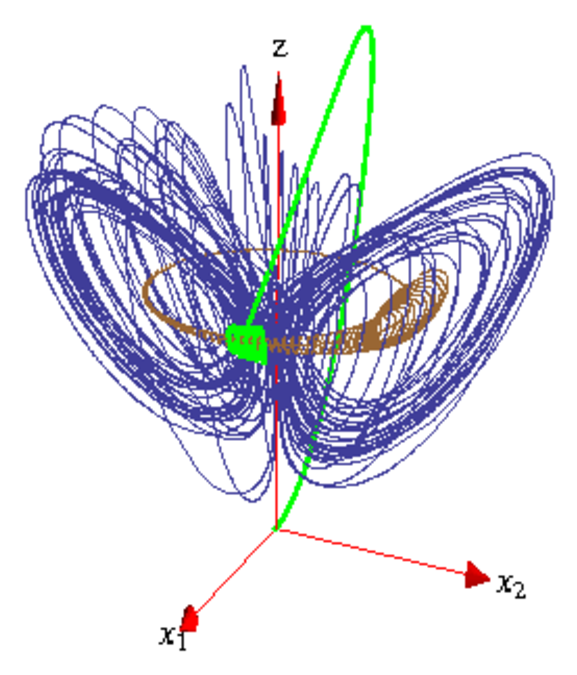
\includegraphics[height=0.25\textheight]{../figs/CLE.eps}
\end{center}
\caption[Complex Lorenz system phase space]
{ \Statesp\ portrait of \CLe\ dynamics for $r_1=28,\, b=8/3,\,
\sigma=10,\, a=1\, e=1/10,\, r_2=0$. Plotted are \reqv\
\REQB{1}(red), it's unstable manifold(brown), \eqv\ \EQB{0}, a
representative of it's unstable manifold(green), 3 repetitions
of \rpo\ ``01''(magenta) and a generic orbit(blue).}
\label{fig:CLE}
\end{figure}
%%%%%%%%%%%%%%%%%%%%%%%%%%%%%%%%%%%%%%%%%%%%%%%%%%%%%%%%%%%%%%%%

To find the location of the relative equilibrium it is convenient to work on polar
coordinates defined by $x=\rho_1 e^{i \phi_1},\,y=\rho_2 e^{i \phi_2}$. Equations \refeq{eq:CLe} with $r_2=0$
take the form
\beq
\begin{split}
	\dot{\rho}_1 &=-\sigma  \rho_1+\sigma \rho_2\cos\Phi \cont
	\dot{\rho}_2 &=-\rho_2 + \rho_1(r_1 -z)\cos\Phi \cont
	\dot{z} &=  -b z+\rho_1 \rho_2\cos\Phi \cont	
	\dot{\Phi} &=-e-\frac{\sigma \rho_2 \sin\Phi}{\rho_1}+\frac{\rho_1(z-\rho ) \sin\Phi }{\rho_2}\,,
	\label{eq:CLePolar}
\end{split}
\eeq
where $\Phi=\phi_1-\phi_2$ and the evolution equations for $\phi_1,\phi_2$ are given by
\beq
\begin{split}
	\dot{\phi}_1 &=-\frac{\sigma \rho_2 \sin\Phi}{\rho_1}\cont
	\dot{\phi_2} &= \frac{e \rho_2+\rho_1 (r_1 -z)\sin\Phi}{\rho_2}\,.
	\label{eq:CLeAngl}
\end{split}
\eeq
The condition for a \reqv~ is that all time derivatives in \refeq{eq:CLePolar} vanish from which we get
% Explicit form here, simplified in terms of z component below
% \beq
% \begin{split}
% 	z &= -\frac{e^2}{(\sigma +1)^2}+r_1 -1\cont
% 	\rho_2 &= \frac{\sqrt{-b \left(e^2+(\sigma +1)^2\right)\left(e^2-(r_1 -1) (\sigma +1)^2\right)}}{(\sigma+1)^2}\cont
% 	\rho_1 &= \frac{\sqrt{-b \left(e^2-(r_1 -1) (\sigma +1)^2\right)}}{\sigma +1}\cont
% 	\Phi &= -\cos ^{-1}\left(\frac{\sigma +1}{\sqrt{e^2+(\sigma +1)^2}}\right)
% \end{split}
% \eeq
\beq
\begin{split}
	z^{(1)} &= \frac{-e^2+(r_1 -1)(\sigma +1)^2}{(\sigma +1)^2}\cont
	\rho_2^{(1)} &= \sqrt{b \left(e^2+(\sigma +1)^2\right)z^{(1)}}\cont
	\rho_1^{(1)} &= \sqrt{b z^{(1)}}\cont
	\Phi^{(1)} &= -\cos ^{-1}\left(\frac{\sigma +1}{\sqrt{e^2+(\sigma +1)^2}}\right)
\end{split}
\eeq
Substituting in \refeq{eq:CLeAngl} we get $\dot{\phi}_1=\dot{\phi}_2=e \sigma/(1 + \sigma)\neq 0$ for $e\neq0$
and thus we have indeed a \reqv and not a group orbit of equilibria.

Calculation  in polar coordinates $\rho_1,\rho_2,\Phi,z$ of stability eigenvalues for \REQB{1}
for the set of parameters we use here yields
\beq
	\mu_{1,2}\pm\omega_{1,2}= 0.0938\pm 10.1945i,\, \lambda_3=-11.0009,\, \lambda_4= -13.8534\,.
\eeq



\subsubsection{Invariant Polynomials}


%%%%%%%%%%%%%%%%%%%%%%%%%%%%%%%%%%%%%%%%%%%%%%%%%%%%%%%%%%%%%%%%%%
\begin{figure}[ht]
\begin{center}
  (\textit{a})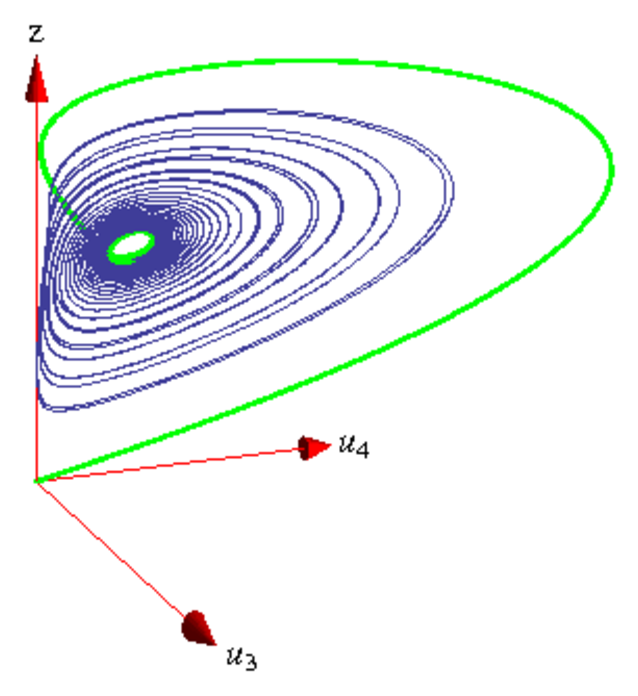
\includegraphics[width=0.35\textwidth]{../figs/CLEip1.eps}
~~~~(\textit{b})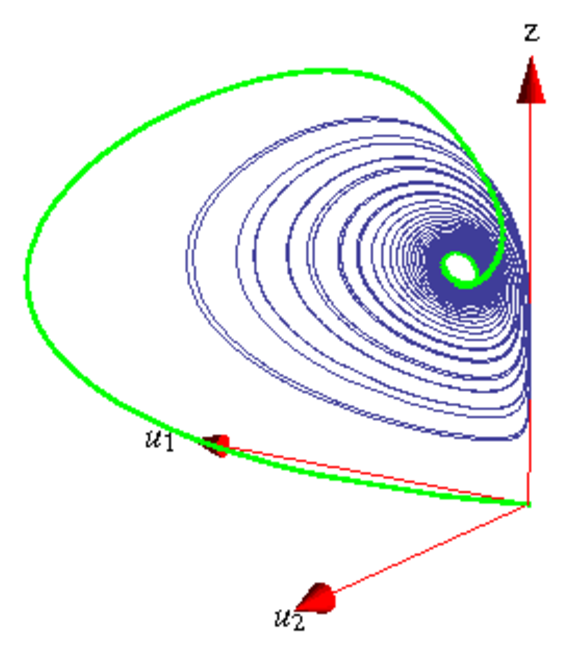
\includegraphics[width=0.36\textwidth]{../figs/CLEip2.eps}
\end{center}
\caption[Orbit space projection of Complex Lorenz system: Invariant polynomials]{ \Statesp\
portraits of \CLe\ dynamics for $r_1=28,\, b=8/3,\, \sigma=10,\, a=1$, $e=1/10$, $r_2=0$
in \reducedsp. Projecting on invariant polynomials \refeq{eq:ipLaser}.
    }
\label{fig:CLEip}
\end{figure}
%%%%%%%%%%%%%%%%%%%%%%%%%%%%%%%%%%%%%%%%%%%%%%%%%%%%%%%%%%%%%%%%

The first approach we try is by use of invariant polynomials \refeq{eq:ipLaser},
following Gilmore and Letellier\rf{GL-Gil07b} who compute invariant polynomials
for the same action of $SO(2)$ and use them for symmetry reduction
of a system conjugate to \CLe s with $e=-r_2$.
For visualization purposes, rather than rewritting the dynamics,
we merelly map the orbits from original coordinates to $u_i$'s, \reffig{fig:CLEip}.
In most projections the folding mechanism is hidden since the dynamics is squeezed near the $z$-axis.
%     \PC{not sure "tearing mechanism" of Gilmore is a good term - noting is
%         torn, it is continuously stretched and then folded with sharp heteroclinic
%         connection edge. {\bf ES:} Agree.}

Nevertheless we can now easily identify a suitable Poincar\'e section, guided
by the Lorenz equations example, as one that contains the z-axis and the relative equilibrium,
defined by the condition $u_1=u_4$\ES{Continue after Lorenz discussion is in place}.

%%%%%%%%%%%%%%%%%%%%%%%%%%%%%%%%%%%%%%%%%%%%%%%%%%%%%%%%%%%%%%%%%%
\begin{figure}[ht]
\begin{center}
  (\textit{a})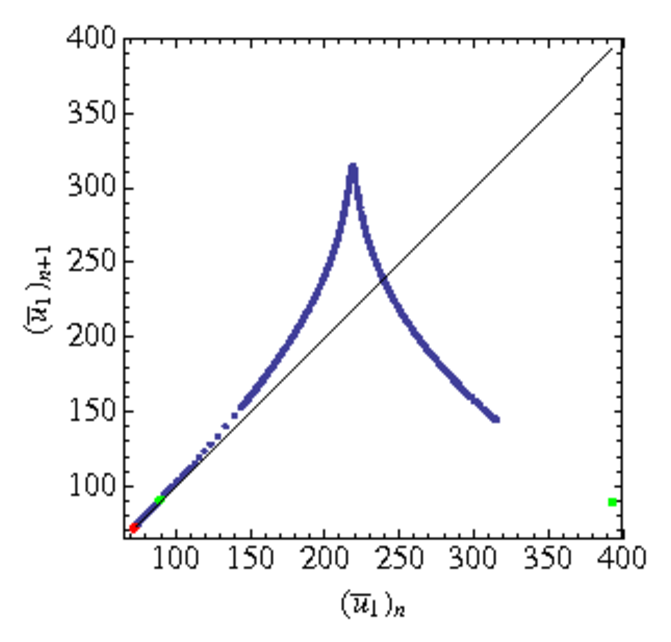
\includegraphics[width=0.35\textwidth]{../figs/CLEipRMu1.eps}
 ~~~~(\textit{b})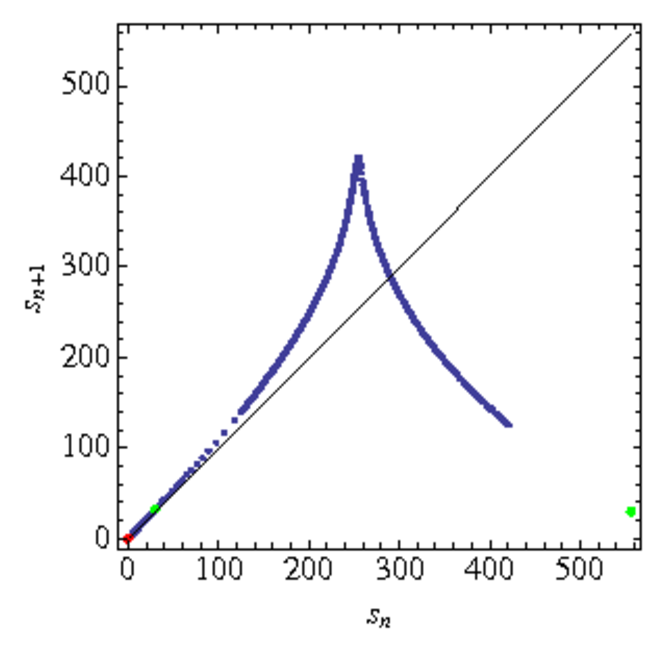
\includegraphics[width=0.35\textwidth]{../figs/CLEipRM.eps}
\end{center}
\caption[\Poincare return map for Complex Lorenz equations, using invariant polynomials]{Return map to the \Poincare
surface of section $u_1=u_4$ for \CLe\ with $r_1=28,\, b=8/3,\, \sigma=10,\, a=1$, $e=1/10$, $r_2=0$,
projecting on invariant polynomials \refeq{eq:ipLaser}. (a) The return map coordinate is
$u_1$, (b) The return map coordinate is the Euclidean
length along the \Poincare section of the unstable manifold of $E_1$.
    }
\label{fig:CLEipRM}
\end{figure}
%%%%%%%%%%%%%%%%%%%%%%%%%%%%%%%%%%%%%%%%%%%%%%%%%%%%%%%%%%%%%%%%

\subsubsection{Moving frame}
\label{sec:CLeMF}


%%%%%%%%%%%%%%%%%%%%%%%%%%%%%%%%%%%%%%%%%%%%%%%%%%%%%%%%%%%%%%%%%%
\begin{figure}[ht]
\begin{center}
  (\textit{a})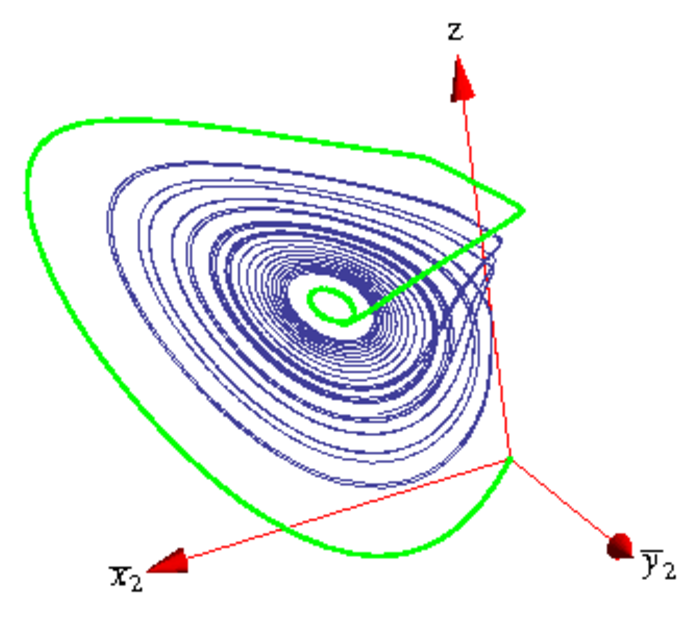
\includegraphics[width=0.35\textwidth]{../figs/CLEmfXYZ.eps}
~~~~(\textit{b})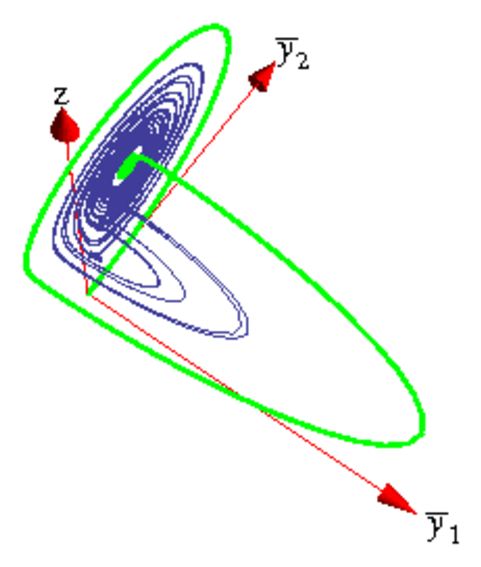
\includegraphics[width=0.35\textwidth]{../figs/CLEmfYYZ.eps}
\end{center}
\caption[Orbit space projection of Complex Lorenz system: Moving frame]{ \Statesp\
portraits of \CLe\ dynamics for $r_1=28,\, b=8/3,\, \sigma=10,\, a=1$, $e=1/10$, $r_2=0$
in \reducedsp. Projecting on invariants given in \refeq{eq:invLaser}.
    }
\label{fig:CLEmf}
\end{figure}
%%%%%%%%%%%%%%%%%%%%%%%%%%%%%%%%%%%%%%%%%%%%%%%%%%%%%%%%%%%%%%%%

As the next choice we explore are the invariants \refeq{eq:invLaser} generated by
the moving frame method.
The action \refeq{eq:SO2act} of $\SOn{2}$ on \Rls{5},
is regular on $\Rls{5}\backslash\{x_1=x_2=y_1=y_2=0\}$. Thus we can define 
a cross-section by, for instance $x_1=0,\,x_2>0$.
We can now construct a moving frame for the action
\refeq{eq:SO2act} of $\SOn{2}$ as follows. We write out
explicitly the group transformations:
\beq
\begin{split}
 	\overline{x}_1 &= x_1 \cos\theta - x_2 \sin\theta\cont
	\overline{x}_2 &= x_1 \sin\theta + x_2 \cos\theta\cont
	\overline{y}_1 &= y_1 \cos\theta - y_2 \sin\theta\cont
	\overline{y}_2 &= y_1 \sin\theta + y_2 \cos\theta\cont	
	\overline{z} &= z\,.
	\label{eq:CLEexplSO2}
\end{split}
\eeq
Then set $\overline{x}_1=0$ and solve
the first of \refeq{eq:CLEexplSO2} for the group parameter to obtain the moving frame
\beq
	\theta=\tan^{-1}\frac{x_1}{x_2}
	\label{eq:CLEmf}
\eeq 
which brings any point  back to the cross-section.\footnote{Implementation note: Here it is important that $\tan^{-1}$ 
distinguishes quadrants on the $(x_1,x_2)$ so the transformation results to the correct geometric
interpretation.} Substituting in the remaining equations we get the invariants
\beq
\begin{split}
	\overline{x}_2 &= \sqrt{x_1^2+x_2^2} \cont
	\overline{y}_1 &= \frac{x_2 y_1-x_1 y_2}{\sqrt{x_1^2+x_2^2}}\cont
	\overline{y}_2 &=\frac{x_1 y_1+x_2 y_2}{\sqrt{x_1^2+x_2^2}}\,.
	\label{eq:invLaser}
\end{split}
\eeq
\ES{The solution $\theta = 2 \tan^{-1}\frac{-x_2+\sqrt{x_1^2+x_2^2}}{x_1}$ was returned by Mathematica. If we use
$\theta = \tan^{-1}\frac{x_2}{x_1}$  without taking care of the quadrant our results are multiplied by $sgn(x_2)$.} 
Notice the relation to the invariant polymials \refeq{eq:ipLaser} and also notice that no syzygy is present.

The projections in \reffig{fig:CLEmf} reveal more about the
topology of the attractor but also present large ``jumps." Notice that
the invariants \refeq{eq:invLaser} are related to the invariant polynomials \refeq{eq:ipLaser}
by division by $\sqrt{x_1^2+x_2^2}$ (except the one that is not present.) This is the
reason we get more clear dynamics: All invariants have the same
``dimensions" as the original coordinates. At the same time division by $\sqrt{x_1^2+x_2^2}$
causes the jumps in the $\overline{y}$ components whenever the magnitude of $x$ comes close to zero.
% Notice that we cannot have $x=0$ for dynamics away the $z$-axis due to the syzygy \refeq{eq:syzLaser}. For, if
% $x=0$ then we would also have $y=0$ and thus we would cross the $z$-axis. This cannot happen
% since the $z$ axis is the fixed point subspace of \SOn{2} and is therefore flow-invariant.

Geometrically we can interpret the jumps in the $\overline{y}$ coordinates as follows: We
have chosen to measure angle on one of the irreducible subspaces of \SOn{2}, the $x$-plane, and project
the dynamics on orbit space by counter-rotating in both irreducible subspaces (the $x$- and $y$-plane.)
As long as a trajectory traces one lobe of the Lorenz attractor the angle varies slowly and no
problem occurs. When a trajectory changes quadrant in the $x$-plane to visit the almost opposite lobe (due to detuning
we don't visit the lobe related by rotation by $\pi$, in reality no such thing exists) we get a rapid
change in angle as the trajectory passes close to the origin. In the $y$-plane we don't necessarily change
quadrant. Call $\Delta \theta_x$ and $\Delta\theta_y$ the change in angle
in the $x$- and $y$-plane respectively, when the trajectory changes quadrant in the $x$ plane.
We always reduce to \reducedsp by correcting by $-\Delta\theta_x$ instead of correcting by the smallest angle\ES{I tried
implementing this directly. No luck.}.

% Since $x$ cannot vanish
The problem is mostly aesthetical in the present case,
but for \KSe\ it will be important to prevent
the denominator from vanishing\ES{Here I have a hunch that the denominator cannot vanish
but I can't prove it}. Since \SOn{2} acts irreducibly in the \CLe\ example
(and also in \KSe) we cannot take more than one irreducible subspace into account
when setting up the normalization equations. We can however restore democracy
between modes by modifying the invariants as follows:
    \PC{replaced ES version
\[\begin{split}
	\overline{x}_2 &= \frac{x_1^2+x_2^2}{\sqrt{x_1^2+x_2^2+y_1^2+y_2^2}} \cont
	\overline{y}_1 &= -\frac{x_2 y_1-x_1 y_2}{\sqrt{x_1^2+x_2^2+y_1^2+y_2^2}}\cont
	\overline{y}_2 &=\frac{x_1 y_1+x_2 y_2}{\sqrt{x_1^2+x_2^2+y_1^2+y_2^2}}\cont
	\overline{z} &=z\,.
	\label{eq:invLaser2}
\end{split}
\]
    }
\beq
\begin{split}
	\overline{x}_2 &= (x_1^2+x_2^2)/r \cont
	\overline{y}_1 &= -(x_2 y_1-x_1 y_2)/r\cont
	\overline{y}_2 &=(x_1 y_1+x_2 y_2)/r\cont
	\overline{z} &=z\cont
	r &= \sqrt{x_1^2+x_2^2+y_1^2+y_2^2}
    \,.
	\label{eq:invLaser2}
\end{split}
\eeq
This set of invariants lacks a geometric interpretation\ES{or does it?} but results in much cleaner phase portraits,
\cf \reffig{fig:CLEinv}.


%%%%%%%%%%%%%%%%%%%%%%%%%%%%%%%%%%%%%%%%%%%%%%%%%%%%%%%%%%%%%%%%%%
\begin{figure}[ht]
\begin{center}
  (\textit{a})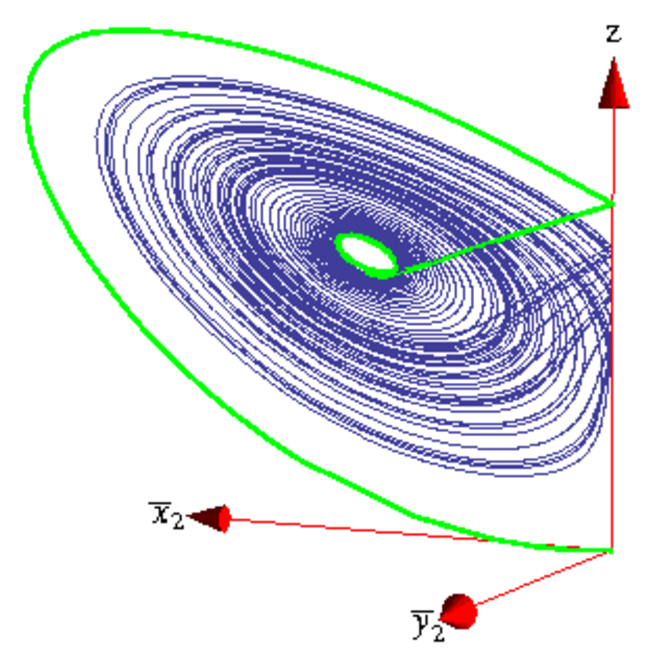
\includegraphics[width=0.35\textwidth]{../figs/CLEinvXYZ.eps}
~~~~(\textit{b})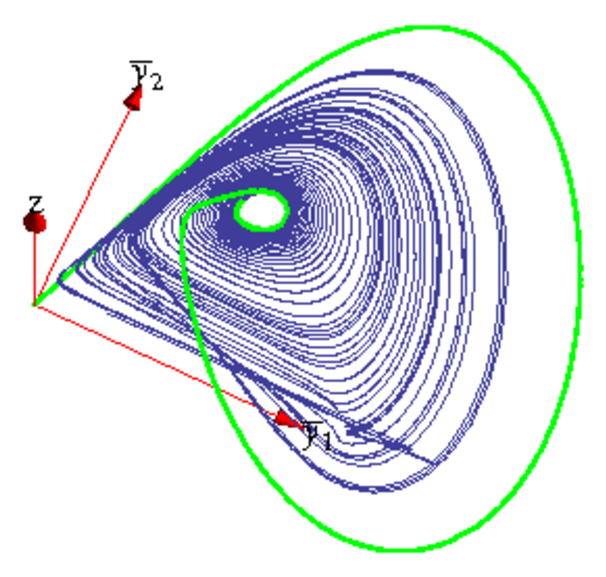
\includegraphics[width=0.35\textwidth]{../figs/CLEinvYYZ.eps}
\end{center}
\caption[Orbit space projection of Complex Lorenz system: Modified moving frame]{ \Statesp\
portraits of \CLe\ dynamics for $r_1=28,\, b=8/3,\, \sigma=10,\, a=1$, $e=1/10$, $r_2=0$
in \reducedsp. Projecting on invariants given in \refeq{eq:invLaser2}.
    }
\label{fig:CLEinv}
\end{figure}
%%%%%%%%%%%%%%%%%%%%%%%%%%%%%%%%%%%%%%%%%%%%%%%%%%%%%%%%%%%%%%%%

%%%%%%%%%%%%%%%%%%%%%%%%%%%%%%%%%%%%%%%%%%%%%%%%%%%%%%%%%%%%%%%%%%
\begin{figure}[ht]
\begin{center}
  (\textit{a})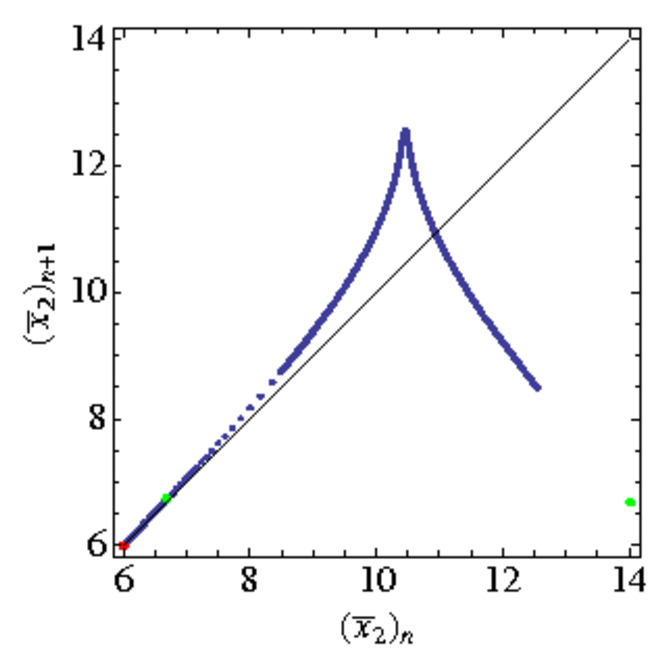
\includegraphics[width=0.35\textwidth]{../figs/CLEinvRMx2.eps}
 ~~~~(\textit{b})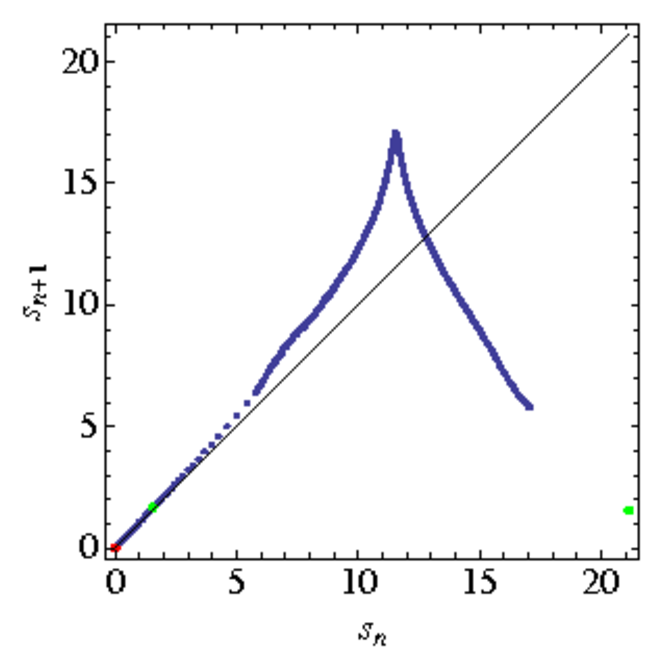
\includegraphics[width=0.35\textwidth]{../figs/CLEinvRM.eps}
\end{center}
\caption[\Poincare return map for Complex Lorenz equations]{Return map to the \Poincare
surface of section $\overline{x}_2=\overline{y}_2$ for \CLe\ with $r_1=28,\, b=8/3,\, \sigma=10,\, a=1$, $e=1/10$, $r_2=0$,
projecting on invariants given in \refeq{eq:invLaser2}. (a) The return map coordinate is
$\overline{x}_2$, (b) The return map coordinate is the Euclidean
length along the \Poincare cross-section of the unstable manifold of $E_1$.
    }
\label{fig:CLEinvRM}
\end{figure}
%%%%%%%%%%%%%%%%%%%%%%%%%%%%%%%%%%%%%%%%%%%%%%%%%%%%%%%%%%%%%%%%


\subsubsection{A geometric approach}

Even though the computation of invariants with the method of the moving coframes is efficient
it is still computationaly prohibitive for high dimensional flows. We will demonstrate
in the example of \CLe\ how one can use the geometric interpretation of the moving coframe method
along with the restriction of the dynamics to a \Poincare section to simply and effectively
perform continuous symmetry reduction in high-dimensional flows.

We have noted that \SOn{2} acts regularly and freely on $X^*=\Rls{5}\backslash\{x_1=x_2=y_1=y_2=0\}$ and
thus we are guaranteed to find the fundamental invariants by the method of moving coframes
if we restrict attention to $X^*$. Nevertheless the transformations \refeq{eq:invLaserRepeat}
obtained by the moving frame method are singular in the subspace $x_1=x_2=0$\ES{Kevin
Mitchell claims that what we do here is geometrically impossible because there is
a non-removable singularity isomorphic to the magnetic monopole string singularity. In
this section I argue that we do not do it globally and this is why it is possible (and we
just do it!)}. Therefore
we would like to ensure that we apply our reduction procedure only on points away from this
subspace. A way to achieve this is by a judicious choice of \Poincare section in original space,
\ie~before reduction. Since we are ultimatelly interested in reducing the dynamics to a \Poincare
return map this is enough for our purposes. Of course locating a \Poincare section is a non-trivial
task on each own right but as we will see in the following, for the procedure to work we will
have to reduce the candidate \Poincare sections to those that are invariant (as a set) under
the group action. Furthermore we already have gained the insight from the simpler \Le problem
that a good choice of section is one that passes through the equilibria that organize the flow.
Here we are naturally led to choose a section that passes through the \reqv~\REQB{1} such as the
section $\mathcal{P}_1$ defined by $\overline{x}_2-\overline{y}_2=0$ in the variables of
\refeq{eq:invLaserRepeat} or by $x_1^2+x_2^2-(x_1 y_1 + x_2 y_2)=0$ in original space and
a suitable orientation condition so that trajectories intersect the section away from
$x_1=x_2=0$ subspace. Here the orientation condition has be chosen so that trajectories intersect
$\mathcal{P}_1$ moving from the ``outside'' of the section in \reffig{fig:CLEmartini} to the
``inside''.
Since $\mathcal{P}_1$ has been chosen to be $\SOn{2}$-invariant, the group orbit of any point on
$\mathcal{P}_1$ lies on $\mathcal{P}_1$. In \reffig{fig:CLEmartini} the group orbits of the points
of intersection of \rpo~``01'' have been visualized as circles on $\mathcal{P}_1$.

The next step is to choose a representative out of each group orbit by means of a section\ES{There is
technical meaning to the word section here.} $\mathcal{P}_2$ that intersects each group orbit
exactly once. The existense of a section is guaranteed since a cross-section as in \refDef{def:cross-section} exists. Here we choose $x_2=0$ for $\mathcal{P}_2$. Geometrically
this is equivalent to rotating each point of intersection on $\mathcal{P}_1$ by
an appropriate angle so that it lies on $\mathcal{P}_2$. This rotation (a linear operation)
can be applied efficiently even in  high dimensional space when the rotation group representation is a direct
sum of irreducible representations, as is frequently the case with truncations of PDE's. 
Globally the transformation is still non-linear through the dependence on the angle.


%%%%%%%%%%%%%%%%%%%%%%%%%%%%%%%%%%%%%%%%%%%%%%%%%%%%%%%%%%%%%%%%%%
\begin{figure}[ht]
\begin{center}
  (\textit{a})\includegraphics[width=0.35\textwidth]{../figs/CLEmartini.eps}
\end{center}
\caption[\CLe desymmetrization with double section]{Use of \Poincare
surface of section $\mathcal{P}_1$ and section $\mathcal{P}_2$ used for symmetry
reduction of \CLe\ dynamics.
$\overline{x}_2=\overline{y}_2$ for \CLe\ with $r_1=28,\, b=8/3,\, \sigma=10,\, a=1$, $e=1/10$, $r_2=0$.
Group orbits of the points of intersection of \rpo\ ``01'' have been visualized as circles.
    }
\label{fig:CLEmartini}
\end{figure}
%%%%%%%%%%%%%%%%%%%%%%%%%%%%%%%%%%%%%%%%%%%%%%%%%%%%%%%%%%%%%%%%
